% !TeX root = ../Masterarbeit.tex
\graphicspath{{kap01/figures/}{./figures/}}
\section{The Problem of Optimization Under Uncertainty}\label{ch:problem}
Engineering decisions must satisfy constraints under conditions that are only partly known when the decision is made. A dispatch schedule must cover uncertain net demand, and a descent trajectory must satisfy terminal conditions despite disturbances. Optimizing against a nominal forecast does not quantify the probability of failure, while protection against every admissible disturbance can demand substantial resources. Chance constraints express the required reliability directly. This thesis studies how kernel density estimation (KDE) of constraint residuals turns that probabilistic requirement into a differentiable nonlinear constraint, and what statistical and numerical qualifications accompany the resulting decisions.

\subsection{Where Deterministic Optimization Falls Short}\label{sec:deterministic}
\subsubsection{The mean-value approach and the flaw of averages}\label{ssec:meanvalue}
Let $x\in X\subseteq\mathbb R^n$ denote the decision, $f:X\to\mathbb R$ its objective, and $\xi\in\mathbb R^d$ a random input. The scalar residual $g(x,\xi)$ is defined so that $g(x,\xi)\le0$ means the requirement is satisfied. A nominal formulation replaces $\xi$ by a fixed value $\bar\xi$, often its mean when that mean exists:
\begin{equation}
  \minimize_{x\in X} f(x)
  \quad\text{subject to }g(x,\bar\xi)\le0.
  \label{eq:detNLP}
\end{equation}
This formulation is useful when variability is small relative to available margins, or when its consequences can be incorporated adequately into ordinary operating costs. It provides no reliability level by itself. If the nominal optimum has an active constraint, disturbances on the violating side of that boundary cause failure even though the nominal residual is zero. Moreover, for nonlinear $g$, evaluating the constraint at the mean input need not equal its expected value. These mechanisms underlie the flaw of averages~\citep{savage2009}; their practical severity depends on the residual distribution and the margin at the selected decision.

\subsubsection{A worked dispatch example}\label{ssec:worked}
Consider a single-bus system in which capacity $x$ must cover uncertain net demand $\xi$. With a positive unit capacity cost $c>0$, the nominal decision problem is
\begin{equation}
  \minimize_{x\ge0}cx
  \quad\text{subject to }\bar\xi-x\le0,
  \qquad g(x,\xi)=\xi-x.
  \label{eq:dispatch}
\end{equation}
For illustration, let $\log\xi\sim\mathcal N(\log100,0.18^2)$, with demand measured in MW. The repository figure generator draws $200{,}000$ samples with random seed~7. Its sample mean is approximately $101.65$~MW; choosing that capacity leaves approximately $46.34\%$ of the generated demands uncovered. The empirical $95\%$ quantile is approximately $134.41$~MW. These are reproducible values from a seeded synthetic illustration, rather than measurements from an operating power system or a separate experimental dataset.

For this monotone residual and positive cost, the chance-constrained optimum is the demand quantile $x^\star=F_\xi^{-1}(1-\varepsilon)$. Thus reliability has an explicit capacity cost. The mean and median differ for the skewed lognormal law: the mean-value plan lies at its own empirical shortfall probability, not at $\varepsilon=0.5$. As $\varepsilon$ approaches zero, the population quantile and required capacity diverge because this distribution has unbounded upper support.
\begin{figure}[t]
  \centering
  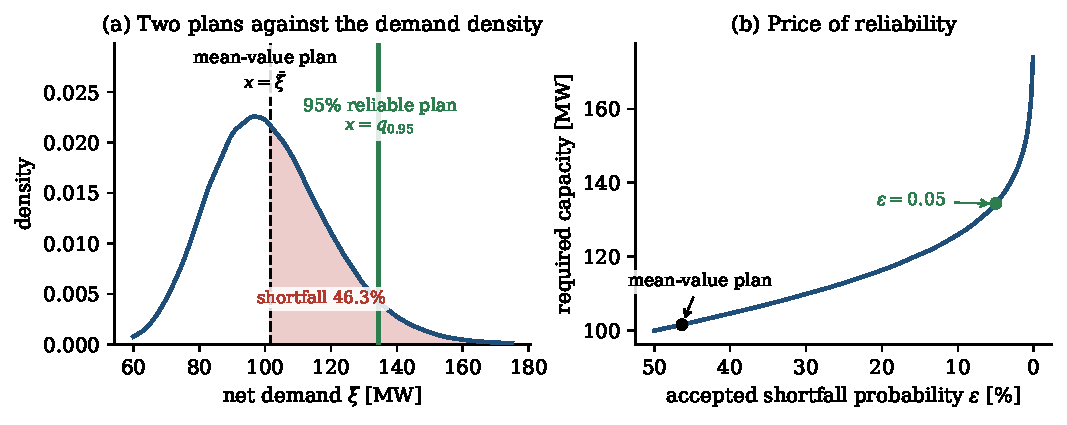
\includegraphics[width=\textwidth]{fig_meanvalue.pdf}
  \caption{Seeded synthetic dispatch illustration. (a) The empirical mean-value capacity and $95\%$ quantile against a KDE of the generated demand samples; shading marks shortfalls for the mean-value plan. (b) Empirical quantile capacity as a function of the accepted shortfall probability, with the mean-value plan located at its measured violation frequency. The curve shows capacity; multiplying by $c$ gives cost.}
  \label{fig:meanvalue}
\end{figure}

\subsubsection{Application contexts}\label{ssec:domains}
The residual formulation connects several application areas. In lunar landing, uncertain dynamics must be reconciled with terminal and path requirements~\citep{keil2021}. In renewable dispatch, uncertain demand and generation enter balance and network constraints~\citep{bienstock2014}. Process planning couples uncertain inputs to production and operating limits~\citep{calfa2015}. Portfolio allocation regulates losses whose distribution can exhibit heavy tails~\citep{cont2001,rockafellar2000}. Each setting requires a decision, a definition of violation, and a distribution against which reliability is assessed. Their disturbance laws and consequences of failure remain application-specific. Chapters~6 and~8 use synthetic dispatch and lunar models to examine the computational mechanisms; process and portfolio applications supply broader motivation, not additional validated case studies.

\subsection{Two Extremes and the Gap Between Them}\label{sec:extremes}
\subsubsection{Ignoring uncertainty and worst-case robustness}\label{ssec:extremes}
Worst-case robust optimization enforces the constraint throughout a prescribed uncertainty set $\Xi$:
\begin{equation}
  g(x,\xi)\le0\quad\text{for all }\xi\in\Xi.
  \label{eq:robust}
\end{equation}
This is appropriate when the set captures the disturbances that must be tolerated and failure within it is unacceptable. Its protection is relative to the chosen set: a bounded set can yield a tractable robust problem even when the underlying probability law has unbounded support~\citep{bental2009}. Enforcing the full support may instead be infeasible, as in finite-capacity dispatch with unbounded demand. A very broad set can also allocate resources to extreme configurations that have little probability. The central modeling decision is therefore which uncertainty and consequences the specification must cover, rather than whether robustness is intrinsically too conservative.

\subsubsection{Chance constraints as a reliability specification}\label{ssec:middleground}
A chance constraint requires
\begin{equation}
  \Prob\{g(x,\xi)\le0\}\ge1-\varepsilon,
  \qquad\varepsilon\in(0,1),
  \label{eq:ccIntro}
\end{equation}
where $\varepsilon$ is the allowed violation probability. Smaller values yield nested, more restrictive feasible sets and cannot improve the optimal objective in a minimization problem with otherwise unchanged data. Unlike an expected penalty, the constraint controls failure frequency directly; it does not control the magnitude of a violation once one occurs. That distinction matters when choosing between probability constraints and tail-risk measures~\citep{shapiro2014,rockafellar2000}.

The limiting zero-risk condition is almost-sure feasibility. It implies protection at every support point when the residual is continuous in the uncertainty; bounded support and further feasibility and regularity conditions are needed to obtain a finite robust limit of the decisions. For the unbounded dispatch example, no finite capacity achieves zero risk. Figure~\ref{fig:spectrum} is therefore a schematic comparison, with its high-reliability endpoint representing a selected bounded uncertainty set. The target setting of this thesis is a specified, nonzero risk budget under data-described uncertainty, potentially outside a convenient parametric family.
\begin{figure}[t]
  \centering
  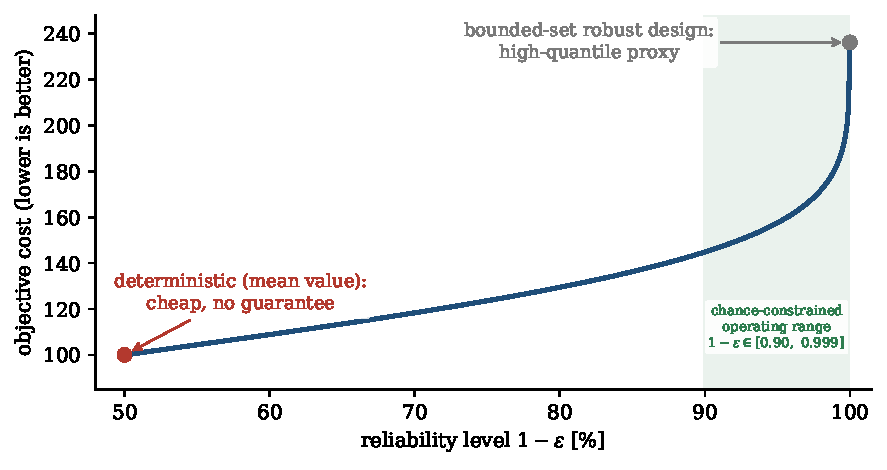
\includegraphics[width=0.82\textwidth]{fig_spectrum.pdf}
  \caption{Schematic cost--reliability comparison. The curve is generated from Gaussian quantiles; its marked high-reliability endpoint is a finite-quantile proxy for protection over a selected bounded uncertainty set, not protection over the full Gaussian support. The shaded band illustrates possible chance-constraint targets.}
  \label{fig:spectrum}
\end{figure}

\subsection{What Chance Constraints Are and Why They Are Hard}\label{sec:hard}
\subsubsection{Individual and joint chance constraints}\label{ssec:definitions}
For a measurable residual $g$, an individual chance constraint has the form
\begin{equation}
  \Prob\{g(x,\xi)\le0\}\ge1-\varepsilon.
  \label{eq:icc}
\end{equation}
For $m$ simultaneous requirements, the joint form is
\begin{equation}
  \Prob\{g_r(x,\xi)\le0,\ r=1,\ldots,m\}\ge1-\varepsilon.
  \label{eq:jcc}
\end{equation}
Separate componentwise constraints with budget $\varepsilon$ do not generally deliver the same joint reliability. A sufficient construction assigns budgets $\varepsilon_r$ satisfying $\sum_{r=1}^m\varepsilon_r\le\varepsilon$ and enforces each component at level $1-\varepsilon_r$. Boole's inequality establishes this allocation without an independence assumption, but overlapping violation events can make it conservative~\citep{prekopa1995}. The individual chance-constrained program is
\begin{equation}
  \minimize_{x\in X}f(x)
  \quad\text{subject to }\Prob\{g(x,\xi)\le0\}\ge1-\varepsilon.
  \label{eq:ccp}
\end{equation}

\subsubsection{Three structural sources of difficulty}\label{ssec:difficulties}
\paragraph{1. Non-convex feasible geometry.}
Even affine scenario constraints can produce a non-convex probabilistic feasible set. With two equally likely scenarios and $\varepsilon=0.5$, satisfying either scenario is sufficient, so the feasible set is the union of their half-spaces. Such a union need not be convex. Convexity is available under additional structure, including suitable joint convexity of the deterministic feasible set and a log-concave uncertainty law~\citep{prekopa1995}. A general nonlinear residual need not satisfy these conditions.

\paragraph{2. Probability evaluation over a moving region.}
Define $S(x)=\{\xi:g(x,\xi)\le0\}$ and the safe probability $p(x)=\Prob\{\xi\in S(x)\}$. If the uncertainty admits a density $\rho_\xi$, then
\begin{equation}
  p(x)=\int_{S(x)}\rho_\xi(u)\,du.
  \label{eq:probability-integral-intro}
\end{equation}
The region changes with the decision, and the density may itself be unknown. Evaluating this integral repeatedly can be demanding even when the density is available, especially in high dimension. When only samples are available, integration and distribution estimation become coupled parts of the optimization problem~\citep{shapiro2014}.

\paragraph{3. Discontinuous empirical indicators.}
Given $N$ independent, identically distributed samples $\xi_1,\ldots,\xi_N$, the direct sample estimate is
\begin{equation}
  \hat p_N(x)=\frac1N\sum_{j=1}^N\ind\{g(x,\xi_j)\le0\}.
  \label{eq:empirical-indicator-intro}
\end{equation}
For a fixed sample, this estimate is constant wherever no residual crosses zero and jumps at crossings. The underlying probability can be smooth even though its empirical approximation is discontinuous. Differentiating the indicator average therefore supplies no useful local information between crossings to a gradient-based solver. Smoothing addresses this computational obstacle, but it also changes the estimated feasible boundary. Figure~\ref{fig:hardness} illustrates the first and third difficulties; the residual transformation below addresses the evaluation structure of the second.
\begin{figure}[t]
  \centering
  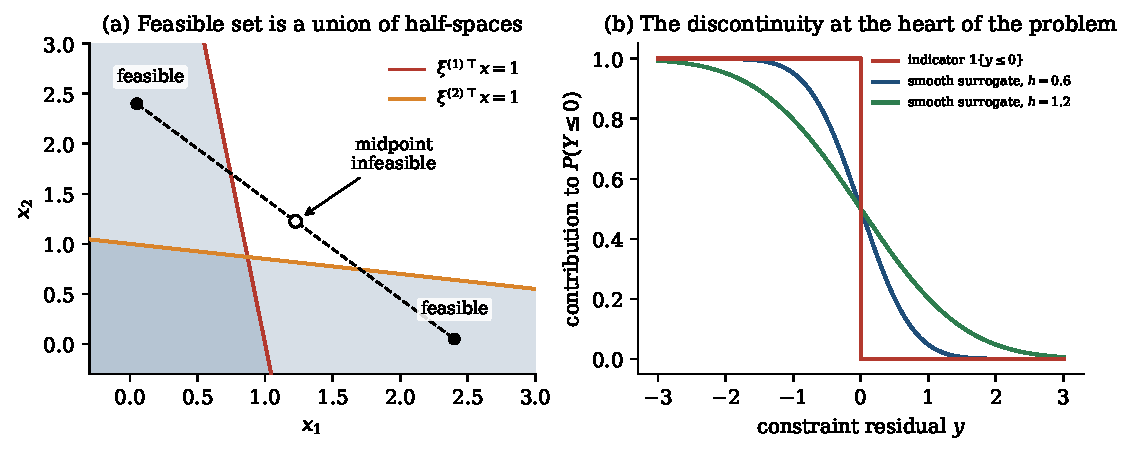
\includegraphics[width=0.9\textwidth]{fig_hardness.pdf}
  \caption{Two structural obstacles. (a) A union of scenario half-spaces gives a non-convex feasible set. (b) A sample indicator and smooth approximations illustrate the transition introduced by smoothing. Smoothing an indicator does not generally convexify the optimization problem.}
  \label{fig:hardness}
\end{figure}

\subsection{Distributional Uncertainty and the Residual-Space Shift}\label{sec:nonparametric}
\subsubsection{Why a parametric law can fail}\label{ssec:parametric}
A parametric law can provide an efficient and interpretable probability model when its assumptions are supported. Reliability calculations, however, depend on the probability mass near and beyond the active threshold. Matching a mean and variance does not establish an accurate tail: skewness, heavy tails, and multiple modes can shift that mass substantially. Misspecification can either understate risk or impose unnecessary conservatism.

Figure~\ref{fig:mismatch} isolates this mechanism using synthetic laws. In its centered Gamma example, the generator's fitted Gaussian assigns approximately $0.23\%$ probability above the marked threshold, while approximately $1.73\%$ of the generated sample lies there. These values demonstrate a particular mismatch, not a universal error factor or an empirical claim about forecast data. KDE reduces commitment to a named distributional family, but finite samples and bandwidth still govern the quality of its tail estimate~\citep{silverman1986}.
\begin{figure}[t]
  \centering
  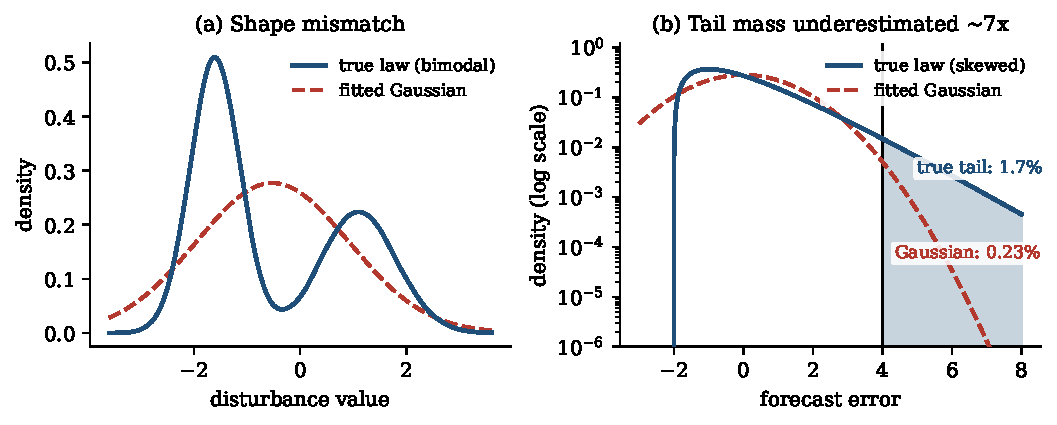
\includegraphics[width=0.82\textwidth]{fig_mismatch.pdf}
  \caption{Synthetic illustrations of distributional misspecification. (a) A KDE of a generated bimodal sample and its moment-matched Gaussian fit. (b) A centered Gamma density and a Gaussian fit to $400{,}000$ generated samples; the annotations compare empirical Gamma and fitted-Gaussian tail probabilities above the marked threshold. Panel~(b) uses random seed~3.}
  \label{fig:mismatch}
\end{figure}

\subsubsection{Estimating residuals rather than uncertainty coordinates}\label{sec:residual}
For a fixed decision $x$, define $Y(x)=g(x,\xi)$ and its cumulative distribution function $F_{Y(x)}$. The identity
\begin{equation}
  F_{Y(x)}(0)=\Prob\{Y(x)\le0\}
  =\Prob\{g(x,\xi)\le0\}=p(x)
  \label{eq:residual-cdf-intro}
\end{equation}
expresses the original safety event without approximation. Suppose $Y(x)$ admits a density. For residual samples $y_j(x)=g(x,\xi_j)$, bandwidth $h>0$, and a nonnegative kernel $K$ integrating to one, its KDE and integrated safe probability are
\begin{equation}
  \hat\rho_h(y;x)=\frac1{Nh}\sum_{j=1}^NK\!\left(\frac{y-y_j(x)}h\right),
  \qquad
  \hat p_h(x)=\int_{-\infty}^0\hat\rho_h(y;x)\,dy.
  \label{eq:kde}
\end{equation}
This is the residual-based construction developed in kernel-smoothed chance-constrained optimization~\citep{calfa2015,schuster2025}.

Three benefits follow. First, the estimated variable is scalar for an individual constraint, regardless of the dimension of $\xi$. Second, the integration region is the fixed half-line $(-\infty,0]$; decision dependence enters through the residual samples. Third, integration yields a finite sum of kernel CDF evaluations that is differentiable in $x$ when the integrated kernel and residual maps have the required smoothness. Chapter~3 derives that sum and its gradient. These benefits concern probability evaluation and solver access; they neither eliminate rare-event sampling requirements nor ensure global convexity.
\begin{figure}[t]
  \centering
  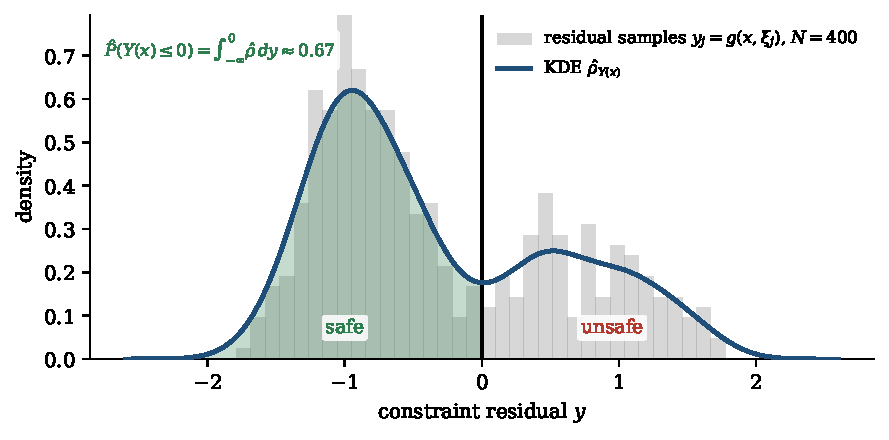
\includegraphics[width=0.88\textwidth]{fig_residual.pdf}
  \caption{Residual-space estimation at a fixed decision, illustrated with $400$ synthetic residual samples. A KDE smooths the histogram, and its mass on the shaded half-line estimates the safe probability. The residual samples change when the decision changes.}
  \label{fig:residual}
\end{figure}

\subsubsection{Bandwidth, one-sided bias, and joint events}\label{ssec:openquestions}
Bandwidth determines both statistical smoothing and the constraint geometry presented to the optimizer. An ordinary symmetric KDE can overestimate the safe probability at finite sample size. A suitably one-sided integrated kernel instead bounds the empirical indicator in the conservative direction. This is a pointwise statement at a fixed decision; transferring it to the unknown probability after selecting a decision from the same data requires additional statistical control or independent validation.

For a joint event, $\max_r g_r(x,\xi)\le0$ is exactly equivalent to satisfying every component. The maximum preserves a scalar statistic but can be nonsmooth in the decision. Chapter~4 studies log-sum-exp smoothing alongside alternative joint constructions, making the additional approximation explicit.

\subsection{Scope and Positioning}\label{sec:scope}
\subsubsection{Positioning relative to anchor work}\label{ssec:positioning}
The thesis connects smooth residual reformulation~\citep{calfa2015}, safety-oriented biased-kernel constructions~\citep{keil2021}, and optimizer-level convergence under explicit assumptions~\citep{schuster2025}. It develops the formulation in Chapter~3, analyzes the local one-sided and joint constructions in Chapter~4, and interprets the convergence conditions in Chapter~5. Chapters~6--8 connect these statements to an implementation and a reproducible validation protocol.

The contribution is an applied optimization analysis and implementation, not a new theorem in KDE theory. The local shifted-Epanechnikov construction is distinguished from Keil's Split--Bernstein kernel and optimal-control workflow. No closed-loop stability or recursive-feasibility result is established, and the synthetic lunar transcription does not by itself certify continuous-time path safety. Statistical statements concern the sampling law; transfer to a changed deployment distribution is outside scope. In particular, asymptotic convergence and empirical test frequencies are not distribution-free finite-sample guarantees for a decision optimized on the training sample.

\subsubsection{Research questions and chapter map}\label{ssec:rqs}
Four research questions organize the analysis:
\begin{enumerate}
  \item \textbf{RQ1: Formulation.} How does residual-space KDE produce a differentiable chance-constraint approximation, and which assumptions justify its estimator, conservative bounds, and optimization limits? Chapters~3--5 provide the mathematical analysis.
  \item \textbf{RQ2: Numerical comparison.} How do nominal, scenario, parametric-reference, and KDE decisions compare in violation probability, objective value, conservatism, and computational behavior where the benchmark supports those measurements? Chapters~7--8 define and report the comparisons.
  \item \textbf{RQ3: Bandwidth and smoothing.} How do bandwidth, one-sided bias, and sample size affect estimated feasibility, held-out violations, and solver behavior? Chapters~4--5 establish the mechanisms, and Chapter~8 reports the diagnostics.
  \item \textbf{RQ4: Joint extension.} How do scalar joint-event statistics and log-sum-exp smoothing compare with alternative constructions, and what conservatism or numerical limitations do they introduce? Chapter~4 develops the extension and Chapter~8 evaluates it.
\end{enumerate}
Chapter~2 supplies the method survey and KDE foundations. Chapter~6 specifies the optimal-control transcription and its audit; Chapters~9--10 interpret the evidence, identify unresolved limitations, and state the supported conclusions.
